\chapter{Introduction}
% ======================================================================================
\section{Motivation}
Fluid-structure interaction (FSI) problems play important role in many scientific and engineering fields, such as automotive, aerospace, and biomedical industry. Despite the wide application, a comprehensive study of FSI systems still remains a challenge due to their strong nonlinearity and multidisciplinary nature. For most FSI problems, analytical solutions to are not available, and physical experiments are limited in scope. Therefore, to get more insight in the physics involved in the complex interaction between fluids and solids, numerical simulations are used. The numerical solutions are conducted based on Computational Fluid Dynamics (CFD) models for the flow and Finite Element Analysis (FEA) for the structural response. Nevertheless, the prohibitive amount of computations has been one of the major issues in the design optimization of such coupled multidisciplinary systems. The other bottle neck is generating an appropriate computational domain that represents the fluid and solid regions. The effort and time required to take a geometry from a CAD package, clean up the model, and generate a mesh is usually a large portion of the overall human time required for the simulation. This cannot be automated for complex and moving domains. The Immersed Boundary (IB) method, reduces the amount of time needed for the fluid flow simulations and provides fast results by directly addressing the challenges associated with this issue.

Due to the large amount of computations involved in the FSI simulation, the gradient based methods are the best candidates for design optimization of such problems. Sensitivity analysis is the integral part of gradient based methods. Although there are analytical techniques for efficient and accurate sensitivity calculation, they have not yet implemented in commercial CFD packages. Therefore, most gradient optimization techniques relay on finite difference method for sensitivity calculation when solving FSI problem that are prone to errors.

The motivation for the research proposed in this document is in two areas. First, we want to have sensitivity analysis capabilities that can treat the solvers as black-box. This means that we can solve both the governing equations and sensitivity response using the same code. Second, a robust analysis technique for the coupled FSI system based on IB method is formulated. The current approach of IB is not suited for the sensitivity analysis due to the discontinuities in its formulation. This will be explained in more details in the following Chapters.

% ======================================================================================
\section{Sensitivity Analysis Overview}
Sensitivity analysis consists of computing the derivatives of solution of the governing equations, i.e. displacement, velocity, or pressure, with respect to one of several independent design variables, i.e. shape of boundaries or size of elements. There various applications for sensitivity information such as improving the accuracy of surrogate models as in gradient enhanced Kriging \cite{han2013improving} or uncertainty quantification \cite{pettit2004uncertainty}. However, our main motivation is the use of this information in gradient-based optimization. The calculation of gradients is often the most expensive step in the optimization cycle therefore, using efficient methods for accurate calculation of sensitivities are vital to the optimization process. As shown in Figure \ref{fig:C1_sensitivityTaxonomy}, methods for sensitivity calculation can be put into three methods: i) numerical, ii) analytical, and iii) automatic differentiation.

\begin{figure}[h]
	\centering
	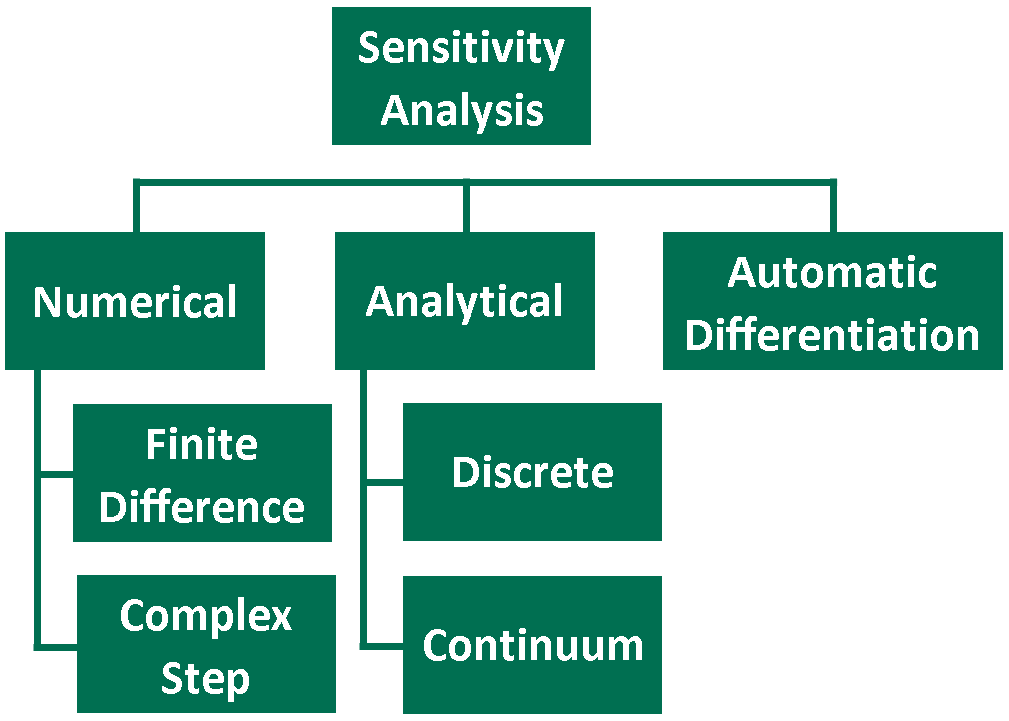
\includegraphics[height=7.00cm]{Chapter_1/figure/sensitivity_taxonomy.png}
	\caption{Sensitivity calculation techniques.}
	\label{fig:C1_sensitivityTaxonomy}
\end{figure}

The Finite Difference (FD) method is probably the easiest method to implement for calculating the sensitivity of a variable. The fact that they can be implemented even when a given computational model is a black box makes most gradient based optimzation algorithms perform finite differences by default when the used does not provide the required gradients. However, the computational cost associated with finite difference for large systems can become very large. For a system with $n$ number of design variables, the analysis needs to be done $n+1$ time to calculate the design sensitivities. Furthermore, to ensure the accuracy, convergence study needs to be done for selecting the appropriate step size for finite difference. The inaccuracy of finite differencing could result in convergence difficulties and inaccurate optimum results. On the other hand, Complex Step (CS) method avoids the loss of precision in finite differences approximation of sensitivities by employing complex arithmetic \cite{martins2003complex}. The complex step derivative is calculated as shown in Equation \eqref{eq:C1_compelxStepFormula}.

\begin{equation}\label{eq:C1_compelxStepFormula}
	\mathcal{F}^\prime\left(u; b\right) = \frac{\text{Im}\left[ \mathcal{F}\left(u; b + ih\right) \right]}{h}
\end{equation}

This means that we perturb the design variable by an imaginary value of $ih$ and then look at
the imaginary portion of the resulting response. Using the complex step method, we can choose a
small step size for $h$ without loosing accuracy. However, many commercial packages such as ANSYS or Nastran cannot handle complex arithmetic which makes the implementation of complex step method infeasible. Moreover, the high cost of finite difference is still associated with the complex method as well.

Automatic differentiation (AD) is based on the systematic application of the differentiation to computer programs \cite{naumann2012art}. In the AD approach, the chain rule of differentiation is applied to every line in the program. This assumes that the computer program consists of a sequence of explicit functions that act successively on some variables. Therefore, by differentiating each of these functions and applying the chain rule, it is possible to calculate the sensitivities. 

There has been many research on utilizing AD for optimization. Bischof et al. used AD for calculating the sensitivities using a CFD solver. They used ADIFOR for differentiating the source code of their CFD code (TLNS3D) which later used for calculating the sensitivity of a transonic flow to change in the boundary conditions. Hascout et al., also used AD for a sonic boom reduction under a supersonic aircraft. However, in all of these works, it is needed to have access to the source code and modify the solver extensively to calculate the sensitivities. This make the use of this method for general purpose codes infeasible since the source code is usually not available.

The short comings of numerical and AD techniques, fuels the research for more sophisticated methods for sensitivity calculation which are generally known as analytical methods. Formulation of the analytical sensitivities requires derivation of analytic sensitivity equations. These are obtained by differentiating the governing equations with respect to design variables such as shape of the boundaries. Analytical methods can be further categorized based on how the sensitivity equations derived and solved. Typically the continuum equations are solved using an approximate method which discretizes the governing equations. The Discrete Sensitivity Analysis (DSA) technique, differentiates the discretized governing equations with respect to design variables to get the analytical sensitivity equations \cite{choi2006structural}. This system of equations is later solved for analytical sensitivities. On the other hand, Continuum Sensitivity Analysis (CSA) takes an alternative approach. The sensitivity equations are derived by differentiating the continuum governing equations and then discretized to be solved. This results in linear Continuous Sensitivity Equations (CSEs), that govern the sensitivity response of the system.

The discrete sensitivity analysis has been historically the method of choice to calculate the high-accurate sensitivity when the details of analysis are available \cite{arora1979methods}. This method has been adopted by the structural optimization community, and been applied to fluid-solid interaction problems as well. Reuther et al., used the discrete method for aerodynamic shape optimization of a complex aircraft configuration \cite{reuther1999constrained}. They used Euler flow as the aerodynamics theory where they optimized different configurations for transonic and supersonic regimes. However, they only focused on the flow. Martins et al., developed an adjoint method for sensitivity analysis for an aero-structural aircraft design framework where the sensitivities were computed using a coupled adjoint approach. The framework was used on a supersonic business jet. In their work, the discretization details of the solver needs to be known to calculate the sensitivities. Source code modification is essential in all the other related research in the area as well


%In Most analysis programs, after discretization, the response, i.e. displacement, velocity, or pressure,  is related to applied load/boundary conditions through stiffness matrix. Therefore, the response sensitivity, depends on the sensitivity of the stiffness matrix. This can calculated by either analytically differentiate the stiffness matrix, or approximate this derivative using finite difference method. The later is known as semi-analytic method and it has advantages and disadvantages as FD method. 